\chapter{Trigonometry}

{\color{blue} This should all be ignored. I was wondering what a rigorous geometric development of sine and cosine would look like (ie, a development that does not begin with power series, but tries to formalize angles and triangles and so forth). Supposedly this used to be common in earlier times but has fallen out of fashion lately. I'm not sure why. These are some incomplete thoughts about this.  }

\section{Arclength function}

\newcommand{\len}{\mathrm{len}}
\newcommand{\arclen}{\mathrm{arclen}}

Let $S^1 = \{ (x, y) : x^2 + y^2 = 1 \}$ be the unit circle inside $\R^2$. We say that a finite list of points in $S^1$ is in \emph{counterclockwise order} if all the points with $y \geq 0$ precede the points with $y < 0$, the points with $y \geq 0$ have decreasing $x$-coordinates, and the points with $y < 0$ have increasing $x$-coordinates. Also, we say that $b$ is \emph{counterclockwise of} $a$ if the list $a, b$ is in counterclockwise order. This defines a total order on $S^1$. 

If $P$ is a finite list of points $a_0, \dotsc, a_n$ in counterclockwise order, we define $\len(P)$ to be the sum of the euclidean distances from $a_{i-1}$ to $a_i$ for all $i = 1, \dotsc, n$. See \cref{circle-length-of-list}. If we add a point to the list $P$ in the appropriate spot to get a new list $P'$ that is still in counterclockwise order, then $\len(P) \leq \len(P')$ by the triangle inequality. 

\begin{figure}[ht]
	\begin{center}
		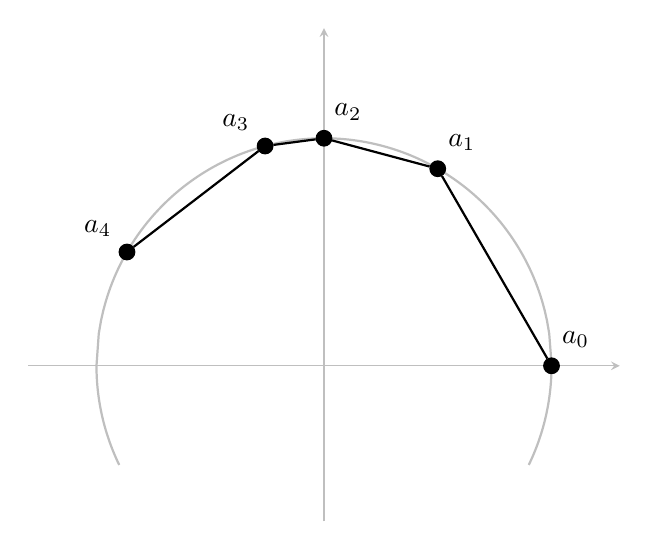
\begin{tikzpicture}
		\begin{axis}[
		xmin=-1.3,xmax=1.3,
		ymin=-0.5,ymax=1.3,
		ytick={-1,1},
		xtick={-1,1},
		xticklabels={},
		yticklabels={},
		axis lines=middle,
		axis line style=lightgray,
		width=0.75\textwidth,
		axis equal,
		]
		
		\addplot[lightgray,style=thick,-] expression[domain=-1:1,samples=200]{sqrt(1-x^2)}; 
		\addplot[lightgray,style=thick,-] expression[domain=0.9:1,samples=200]{-sqrt(1-x^2)};
		\addplot[lightgray,style=thick,-] expression[domain=-1:-0.9,samples=200]{-sqrt(1-x^2)};
		
		
		\node[label={85:{$a_0$}},color=black,draw=black,circle,fill,inner sep=2pt] at (axis cs:1,0) (A) {}; 
		\node[label={85:{$a_1$}},color=black,draw=black,circle,fill,inner sep=2pt] at (axis cs:0.5,0.866025) (B) {}; 
		\node[label={85:{$a_2$}},color=black,draw=black,circle,fill,inner sep=2pt] at (axis cs:0,1) (C) {}; 
		\node[label={135:{$a_3$}},color=black,draw=black,circle,fill,inner sep=2pt] at (axis cs:-0.258819,0.965926) (D) {};
		\node[label={135:{$a_4$}},color=black,draw=black,circle,fill,inner sep=2pt] at (axis cs:-0.866025,0.5) (E) {}; 
		
		\draw[black, thick] (A) -- (B) -- (C) -- (D) -- (E);
		
		\end{axis}
		\end{tikzpicture}
	\end{center}
	\caption{Given a list of points $P = a_0, \dotsc, a_n$ in counterclockwise order, we define $\len(P)$ to be the sum of the euclidean distatnces between $a_{i-1}$ to $a_i$ for all $i = 1, \dotsc, n$. In the picture above, this is the total length of the line segments between the points.}  \label{circle-length-of-list}
\end{figure}

Given a point $a \in S^1$, a \emph{partition of the arclength from $(1,0)$ to $a$} is a finite list of points $a_0, \dotsc, a_n$ in counterclockwise order with $a_0 = (1,0)$ and $a_n = a$. We then define
\[ \arclen(a) = \sup \{ \len(P) : P \text{ is a partition of the arclength from } (1,0) \text{ to } a \}. \] 
Notice that $\arclen(1,0) = 0$ and $\arclen(a) \geq 0$ for all $a$. \Cref{arclength-finite} shows that $\arclen(a)$ is a  finite real number, so we have defined a function $\arclen : S^1 \to \R$. 

\begin{lemma} \label{arclength-finite}
	For any $a \in S^1$, we have $\arclen(a) \leq 8$. 
\end{lemma}

\begin{proof}
	Let $(1, 0) = a_0, \dotsc, a_n$ be a list in counterclockwise order. It is sufficient to show that 
	\begin{equation} \label{inscribed-polygon-perimeter} |a_0 - a_1|_2 + \dotsb + |a_{n-1} - a_n| + |a_n - a_0| \leq 8. \end{equation}
	Geometrically, this assertion says that the perimeter of any polygon inscribed inside the unit circle is at most 8. By the triangle inequality, inserting points into the list $a_0, \dotsc, a_n$ increases the left hand side of inequality \ref{inscribed-polygon-perimeter}. So, to prove \cref{inscribed-polygon-perimeter}, we can assume without loss of generality that the four points $(\pm 1, 0), (0, \pm 1)$ all show up in the list $a_0, \dotsc, a_n$. If $a_k = (0,1)$, by symmetry it is sufficient to show that 
	\[ |a_0 - a_1| + \dotsb + |a_{k-1} - a_k| \leq 2. \]
	This follows from the triangle inequality. See \cref{arclength-finite-picture}. 
	\begin{figure}[ht]
		\begin{center}
			\begin{tikzpicture}
			\begin{axis}[
			xmin=-0.2,xmax=1.1,
			ymin=-0.2,ymax=1.1,
			ytick={-1,1},
			xtick={-1,1},
			xticklabels={},
			yticklabels={},
			axis lines=middle,
			axis line style=lightgray,
			width=0.75\textwidth,
			axis equal
			]
			
			\addplot[lightgray,style=thick,-] expression[domain=-0.1:1,samples=200]{sqrt(1-x^2)}; 
			\addplot[lightgray,style=thick,-] expression[domain=0.9:1,samples=200]{-sqrt(1-x^2)};
			
			\node[label={45:{$a_0$}},color=black,draw=black,circle,fill,inner sep=2pt] at (axis cs:1,0) (A) {}; 
			\node[label={85:{$a_1$}},color=black,draw=black,circle,fill,inner sep=2pt] at (axis cs:0.5,0.866025) (B) {}; 
			\node[label={85:{$a_2$}},color=black,draw=black,circle,fill,inner sep=2pt] at (axis cs:0.258819,0.965926) (C) {};
			\node[label={135:{$a_3$}},color=black,draw=black,circle,fill,inner sep=2pt] at (axis cs:0,1) (D) {}; 
			
			
			\node[inner sep=0pt] at (axis cs:1,0.866025) (E) {}; 
			\node[inner sep=0pt] at (axis cs:0.5,0.965926) (F) {}; 
			\node[inner sep=0pt] at (axis cs:0.258819,1) (G) {};
			
			\draw[black, thick] (A) -- (B) -- (C) -- (D);
			
			\draw[black, dashed] (A) -- (E) -- (B) -- (F) -- (C) -- (G) -- (D);
			
			\end{axis}
			\end{tikzpicture}
		\end{center}
		\caption{If $(1,0) = a_0, \dotsc, a_k= (0,1)$ is list in counterclockwise order, then the sum of the euclidean distances is the total length of the black lines drawn above. This is at most the sum of the lengths of the vertical and horizontal dashed lines, by the triangle inequality. Since the total vertical length of the dashed lines is 1 and so is the total horizontal length, we conclude that the sum of the euclidean distances is at most $2$.}  \label{arclength-finite-picture}
	\end{figure}
\end{proof}

\begin{lemma} \label{arclen-strictly-increasing}
	$\arclen$ is an injective function. In fact, if $b$ is counterclockwise of $a$ and $b \neq a$, then $\arclen(b) > \arclen(a)$. 
\end{lemma}

\begin{proof}
	Suppose $P$ is a partition of the arclength from $(1,0)$ to $a$. Tacking on $b$ yields a new list $P'$ that is a partition of the arclength from $(1,0)$ to $b$, so
	\[ \len(P) + |b-a|_2 = \len(P') \leq \arclen(b). \]
	Taking the supremum over all $P \in \mathscr{P}(a)$ shows that 
	\[ \arclen(a) + |b-a|_2 \leq \arclen(b). \]
	In particular, $\arclen(a) < \arclen(b)$. 
\end{proof}

\begin{remark} \label{taxicab-norm}
	In the following proof, we will use the \emph{$L^1$ norm} or the \emph{taxicab norm} on $\R^2$. It is defined by 
	\[ |(x,y)|_1 = |x| + |y|. \]
	Observe that for any $a  \in \R^2$,  
	\[ |a|_2 \leq |a|_1 \leq \sqrt{2}|a|_2. \]
	Moreover, if $a$ and $b$ are two points in $\R^2$ in the same quadrant (where points on coordinate axes are considered to be in all quadrants they are contiguous to), then 
	\[ |a|_1 + |b|_1 = |a+b|_1. \]
\end{remark}

\begin{lemma} \label{arclen-continuous}
	$\arclen$ is continuous away from $(1,0)$. 
\end{lemma}

\begin{proof}
	Suppose $a, b \neq (1,0)$ are in the same quadrant of the plane (where points on the axes are considered to be in both quadrants they are contiguous to), and that $b$ is  counterclockwise of $a$. Fix $\epsilon > 0$. Let $P$ be a partition of the arclength from $(1,0)$ to $a$ such that $\arclen(a) - \len(P) \leq \epsilon$. 
	
	Let $Q$ be a partition of the arclength from $(1,0)$ to $b$ such that $\arclen(b) - \len(Q) \leq \epsilon$. If $Q'$ is the partition of the arclength from $(1,0)$ to $b$ obtained by merging $P$ and $Q$, observe that $\len(Q) \leq \len(Q')$, so $\arclen(b) - \len(Q') < \epsilon$ also. Thus we can replace $Q$ with $Q'$ in order to assume that $P$ is a sublist of $Q$. 
	
	Let $R = a_0, \dotsc, a_m$ be the sublist of $Q$ starting from $a_0 = a$ and ending with $a_m = b$, so that $\len(P) + \len(R) = \len(Q)$. Then 
	\[ \len(R) \leq |a_0 - a_1|_1 + \dotsb + |a_{m-1} - a_m|_1 = |b-a|_1 \leq \sqrt{2}|b-a|_2, \]
	using \cref{taxicab-norm}. For the equality in the middle, we have used the fact that since $a$ and $b$ are in the same quadrant, all of the points $a_0 - a_1, a_1 - a_2, \dotsc, a_{m-1} - a_m$ are also in the same quadrant. Thus
	\[ 0 \leq \arclen(b) - \arclen(a) \leq \len(Q) - \len(P) + 2\epsilon = \len(R) + 2\epsilon \leq \sqrt{2}|b-a|_2 + 2\epsilon. \]
	Letting $\epsilon \to 0^+$, we find that 
	\[ 0 \leq \arclen(b) - \arclen(a) \leq \sqrt{2}|b-a|_2, \]
	which proves that $\arclen$ is continuous. 
\end{proof}

\section{Definition of \texorpdfstring{$\pi$}{pi}}

\begin{definition}
	We define $\pi$ to be the unique positive real number with  the property that 
	\[ 2\pi = \sup \arclen(S^1). \]
	We know from \cref{arclength-finite} that this supremum is finite. 
\end{definition}

\begin{lemma}
	$\arclen(S^1) = [0, 2\pi)$. 
\end{lemma}

\begin{proof}
	Let $U = S^1 \setminus \{(1,0)\}$. Then $U$ is connected and $\arclen|_U$ is continuous, so $\arclen(U)$ is an interval. It is clear that $\inf \arclen(U) = 0$, and we know that $\arclen(1,0) = 0$, so $0 \in \arclen(S^1)$. Now \[ 2\pi = \sup \arclen(S^1) = \sup \arclen(U). \]
	If there existed $a \in S^1$ such that $\arclen(a) = 2\pi$, then we could choose a point $b$ which is counterclockwise of $a$ and $b \neq a$. Then $\arclen(b) > \arclen(a) = 2\pi$ by \cref{arclen-strictly-increasing}, contradicting the definition of $2\pi$ as a supremum. Thus $2\pi$ is not in the image of $\arclen$, proving the lemma.  
\end{proof}

\begin{exercise}
	Show that $\pi = \arclen(-1,0)$. 
\end{exercise}

\section{Sine and cosine}

We have seen that $\arclen$ is a bijection $S^1 \to [0, 2\pi)$. We can now define sine and cosine in terms of the inverse function $\arclen^{-1} : [0, 2\pi) \to S^1$.  

\begin{definition}
	For $\theta \in [0, 2\pi)$, we define the \emph{cosine} and \emph{sine} of $\theta$, denoted $\cos(\theta)$ and $\sin(\theta)$, to be the $x$- and $y$-coordinates of $\arclen^{-1}(\theta)$, respectively. In other words,
	\[ \arclen^{-1}(\theta) = (\cos(\theta), \sin(\theta)). \]
	Then, for any $\theta \in \R$, there exists a unique $\theta' \in [0, 2\pi)$ such that $\theta = \theta' + 2\pi k$ for some integer $k$, and we define $\cos(\theta) = \cos(\theta')$ and $\sin(\theta) = \sin(\theta')$. 
\end{definition}

% TODO: Continuity

% TODO: sin x / x

% TODO: angle sum formula for sine

% TODO: cos(x) = sin(pi/2 - x)